% ---
% Arquivo com a execução do Trabalho de Conclusão de Curso dos alunos
% Gabriel Takaoka Nishimura, Felippe Demarqui Ramos e Vivian Kimie Isuyama 
% da Escola Politécnica da Universidade de São Paulo
% ---
	\chapter{Execução}\label{cap-execucao}
	
	\section{Arquitetura}
	
	\begin{figure}[htb]
		\caption{\label{fig_arch} Desenho esquemático}
		\centering
		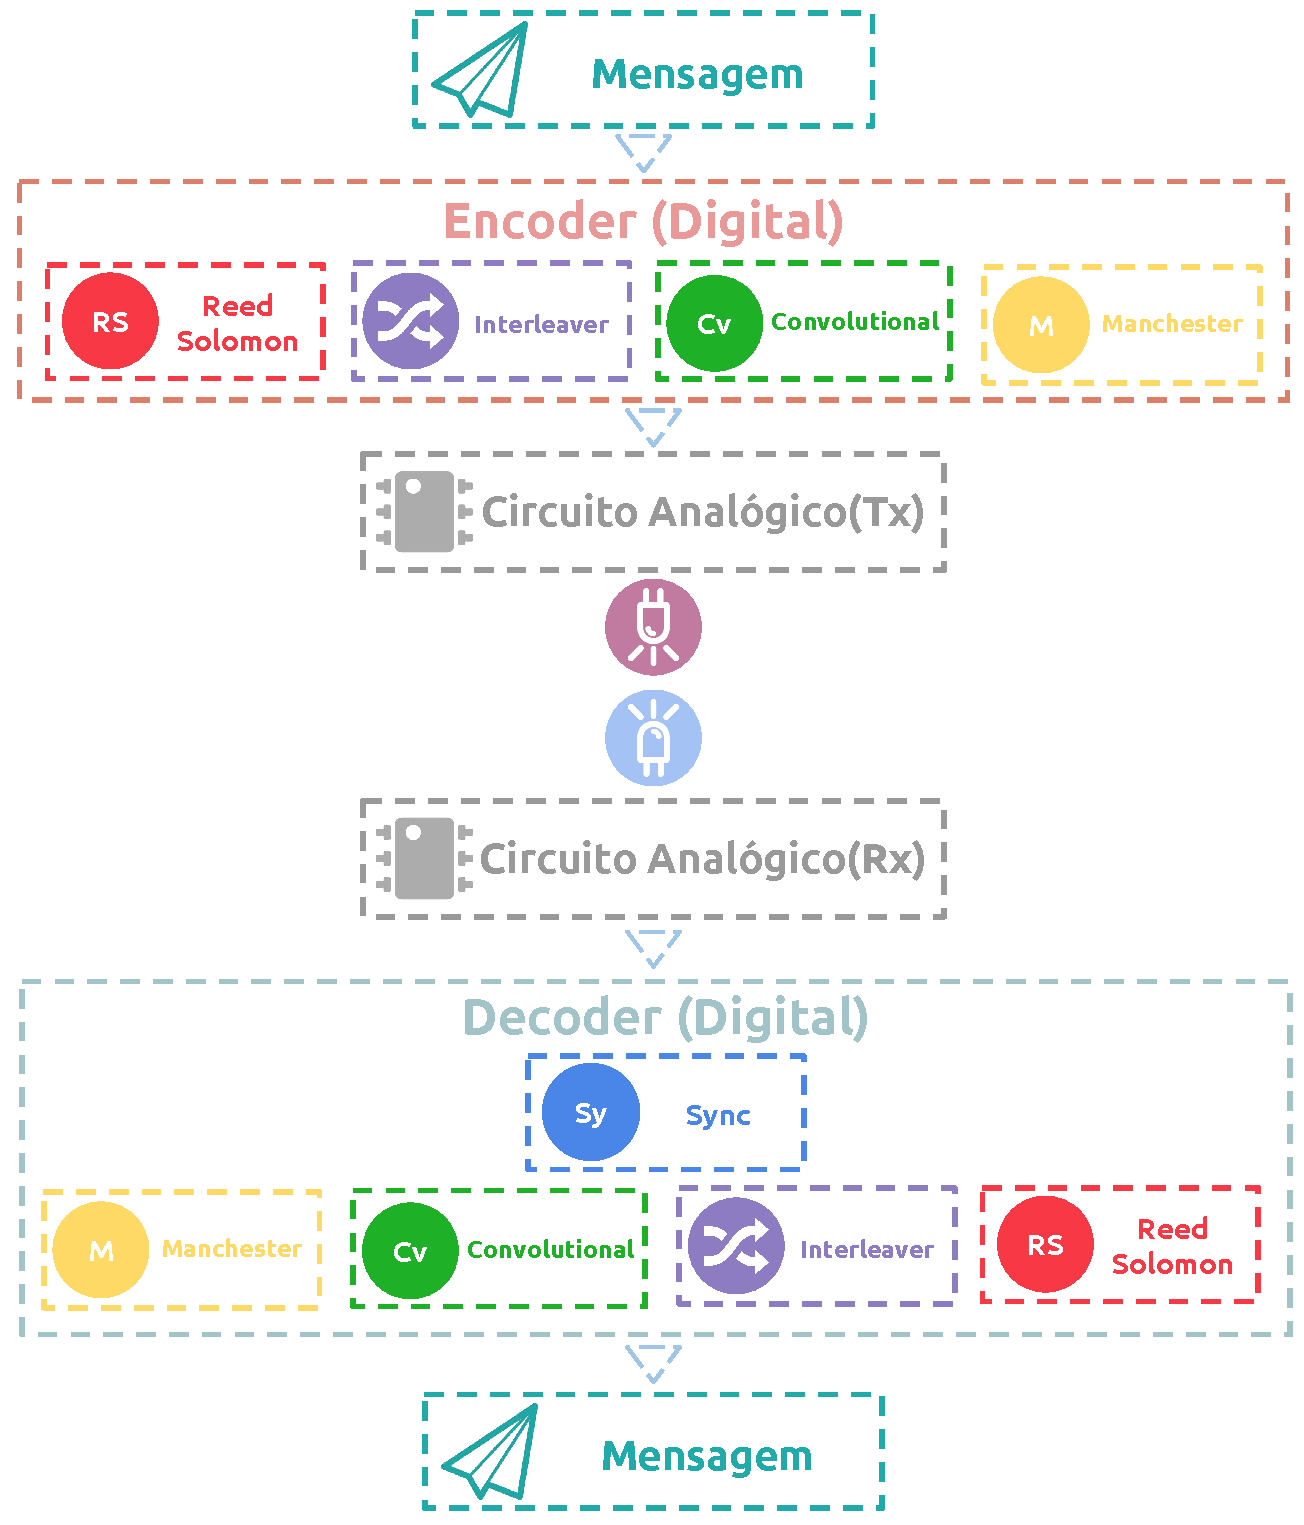
\includegraphics[width=1\textwidth]{Arquitetura}
		\legend{Fonte: Autores.}
	\end{figure}
	
	
	\subsection{Codificador}
	
	Conforme apontado no capítulo de Metodologia, a arquitetura do codificador Reed Solomon foi construída para um código (15, 7), portanto contando com 8 registradores em série. Os multiplicadores foram feitos com uma tabela,  que recebe duas entradas e retorna uma saída, de maneira a simplificar o trabalho de fazer uma função utilizando lógica combinatória. Já os somadores são equivalentes à função de OU exclusivo, ou XOR, com duas entradas e uma saída de 4 bits cada - ou seja, um símbolo. Além destes, os módulos básicos ainda compreendem um multiplexador, que seleciona um entre dois símbolos.
	
	Diagrama do codificador
	
	O comportamento de codificação de uma mensagem pode ser exemplificado pela seguinte simulação, onde se observa a entrada de uma mensagem de 7 símbolos e a saída de um bloco de 15 símbolos, sendo 8 de paridade.
	
	
	\subsection{Decodificador}
	
	A arquitetura do decodificador segue o diagrama funcional da figura X do capítulo de Metologia. Desta forma, o desenvolvimento pode ser separado em quatro partes principais, apresentadas a seguir.
	
	Cálculo das Síndromes
	
	O cálculo das síndromes é feito de forma iterativa, durando tantos ciclos quanto forem os símbolos da mensagem. O cálculo de cada síndrome é independente dos cálculos das demais, e depende apenas dos símbolos de entrada e de cada uma das raízes do polinômio codificador, de alpha0 a alpha7 neste caso.
	
	*diagrama de cálculo das síndromes*
	
	A simulação a seguir representa o caso em que existem erros na mensagem codificada, o que é indicado por síndromes diferentes de 0000.
	
	*simulação das síndromes*
	
	Módulo de Berlekamp-Massey
	
	O módulo de Berlekamp-Massey foi implementado de forma a primeiramente calcular as localizações dos erros, ou seja, os coeficientes do polinômio localizador de erros, representados por Lamba, e guardados em registradores, para o posterior cálculo dos valores dos erros. Os valores de erros são calculados então, com as síndromes e localizações de erro.
	
	Diagrama do módulo
	
	Simulação
	
	% ---
	\section{Hardware}
	% ---
	A seção abaixo discorrerá sobre a aplicação dos métodos estudados nos capítulos anteriores para Hardware.
	Antes de iniciar a execução do trabalho, foram estabelecidas algumas decisões de projeto:
	
	* formato de lista *
	Única fonte de alimentação de 5V.
	Implementação de um circuito apenas para a camada PHY I da norma, fixando a frequência de operação a 200kHz.
	
	. . .
	
	
	\subsection{Transmissor}
	
	\subsubsection{Conversor Digital-Analógico}
		Com os estudos feitos no \autoref{method-hardware-conv-da}, é possível especificar os requisitos reais para o transistor de potência:

		\begin{itemize}
			\item Tensão de base/gate compatível com 3.3V;
			\item Corrente de saída compatível com LED de alta potência, no mínimo 750mA;
			\item Resposta de base/gate a $V_{on(FPGA)}$ de no máximo 1us;
		\end{itemize}
		
		Alguns dos parâmetros são decisões de projeto, como a utilização de níveis TTL para chaveamento do transistor (3.3V ou 5V), e outros são requisitos da norma IEEE, como frequência de operação a 200kHz. Especialmente no segundo caso, é importante escolher um transistor com $T_{rise}$ e $T_{fall}$ de no mínimo 10-100 vezes menor que o período da onda transmitida - no caso $5\mu$$s/100 = 50ns$. Se o transistor não chavear rápido suficiente, é possível que a onda fique alterada. Em alguns casos é possível que fique semelhante a uma onda dente de serra.
		
		O componente escolhido foi um MOSFET de Potência, mais especificamente o IRLZ14, pois é um transistor de nível lógico, pois tem o GATE compatível com voltagens de microcontrolador. 
		
		\begin{figure}[htb]
			\caption{\label{fig_transfer_carac_irlz14} Características de transferência do MOSFET de potência IRLZ14.}
			\centering		%  trim={<left> <lower> <right> <upper>} 
			
\includegraphics[page=3, width=0.7\textwidth, trim={12cm 16.5cm 2.2cm 5cm}, clip]{circuits/irlz14.pdf}
			\legend{Fonte: \cite{datasheet-irlz14}}
		\end{figure}
	
		De acordo com função de transferência da \autoref{fig_transfer_carac_irlz14}, a VGS=3.3V é permitida uma corrente de dreno de 2A. A datasheet também especifica parâmetros de resposta dinâmica do circuito, como seu $T_{rise}$, $T_{fall}$, que estão disponibilizados na tabela abaixo.
		
		\begin{table}[ht]
			\caption{Características Dinâmicas do MOSFET IRLZ14}
			\centering
			\begin{tabular}{c c}
				\hline
				Parâmetro  & Valor  \\ \hline
				$T_{rise}$ & 110 ns \\
				$T_{fall}$ & 26 ns  \\ \hline
			\end{tabular}
			\label{tab_irlz14_timing}
			\legend{Fonte: Vishay Siliconix.}
		\end{table}

	\subsubsection{Transmissão de Luz}
		
		Para realizar a transmissão de luz a distâncias de pelo menos um metro, será necessária a utilização de um LED de potência. Esse LED deverá atender a requisitos de altas frequência e resposta luminosa de acordo com seu chaveamento. Procuranto satisfazer tais parâmetros, o componente escolhido foi da OSRAM, o LUW W5-AM.

		Utilizando o circuito polarizador do LED da \autoref{fig_led_circuit}, é necessário calcular o valor da resistência de $R_{LIMIT}$. O LED permite no máximo 1000mA de corrente de polarização, mas não é desejável trabalhar na região limite de corrente, portanto o circuito será projetado para funcionar a 500mA. Como a voltagem de operação é de 5V, utilizando a Lei de Ohm:
		\begin{equation}
		R_{LIMIT} = 5V \cdot 500mA = 2.5\Omega
		\end{equation}
		
		
	\subsubsection{Versões Anteriores}
		
		Devido a falta de conhecimento do comportamento de transistores e da resposta de todos os componentes a frequência de 200kHz, foram projetados vários circuitos que não satisfaziam o formato de onda desejado. Abaixo são exemplificadas algumas versões implementadas, juntamente com os motivos de terem sido abandonadas.
		
		\paragraph{Filtro da Ponta de Prova}
		
		O primeiro problema que o projeto do transmissor encontrou foi o comportamento de subamortecimento nos terminais do LED. Ele utiliza um circuito semelhante ao utilizado em pontas de provas para filtrar ruídos e é conectado em série com a entrada do transmissor, como visto na \autoref{fig_transmitter_lify_circuit_fail0}.
		
		\begin{figure}[htb]
			\caption{\label{fig_transmitter_lify_circuit_fail0} Circuito de transmissão de dados LiCy.}
			\centering		%  trim={<left> <lower> <right> <upper>} 
			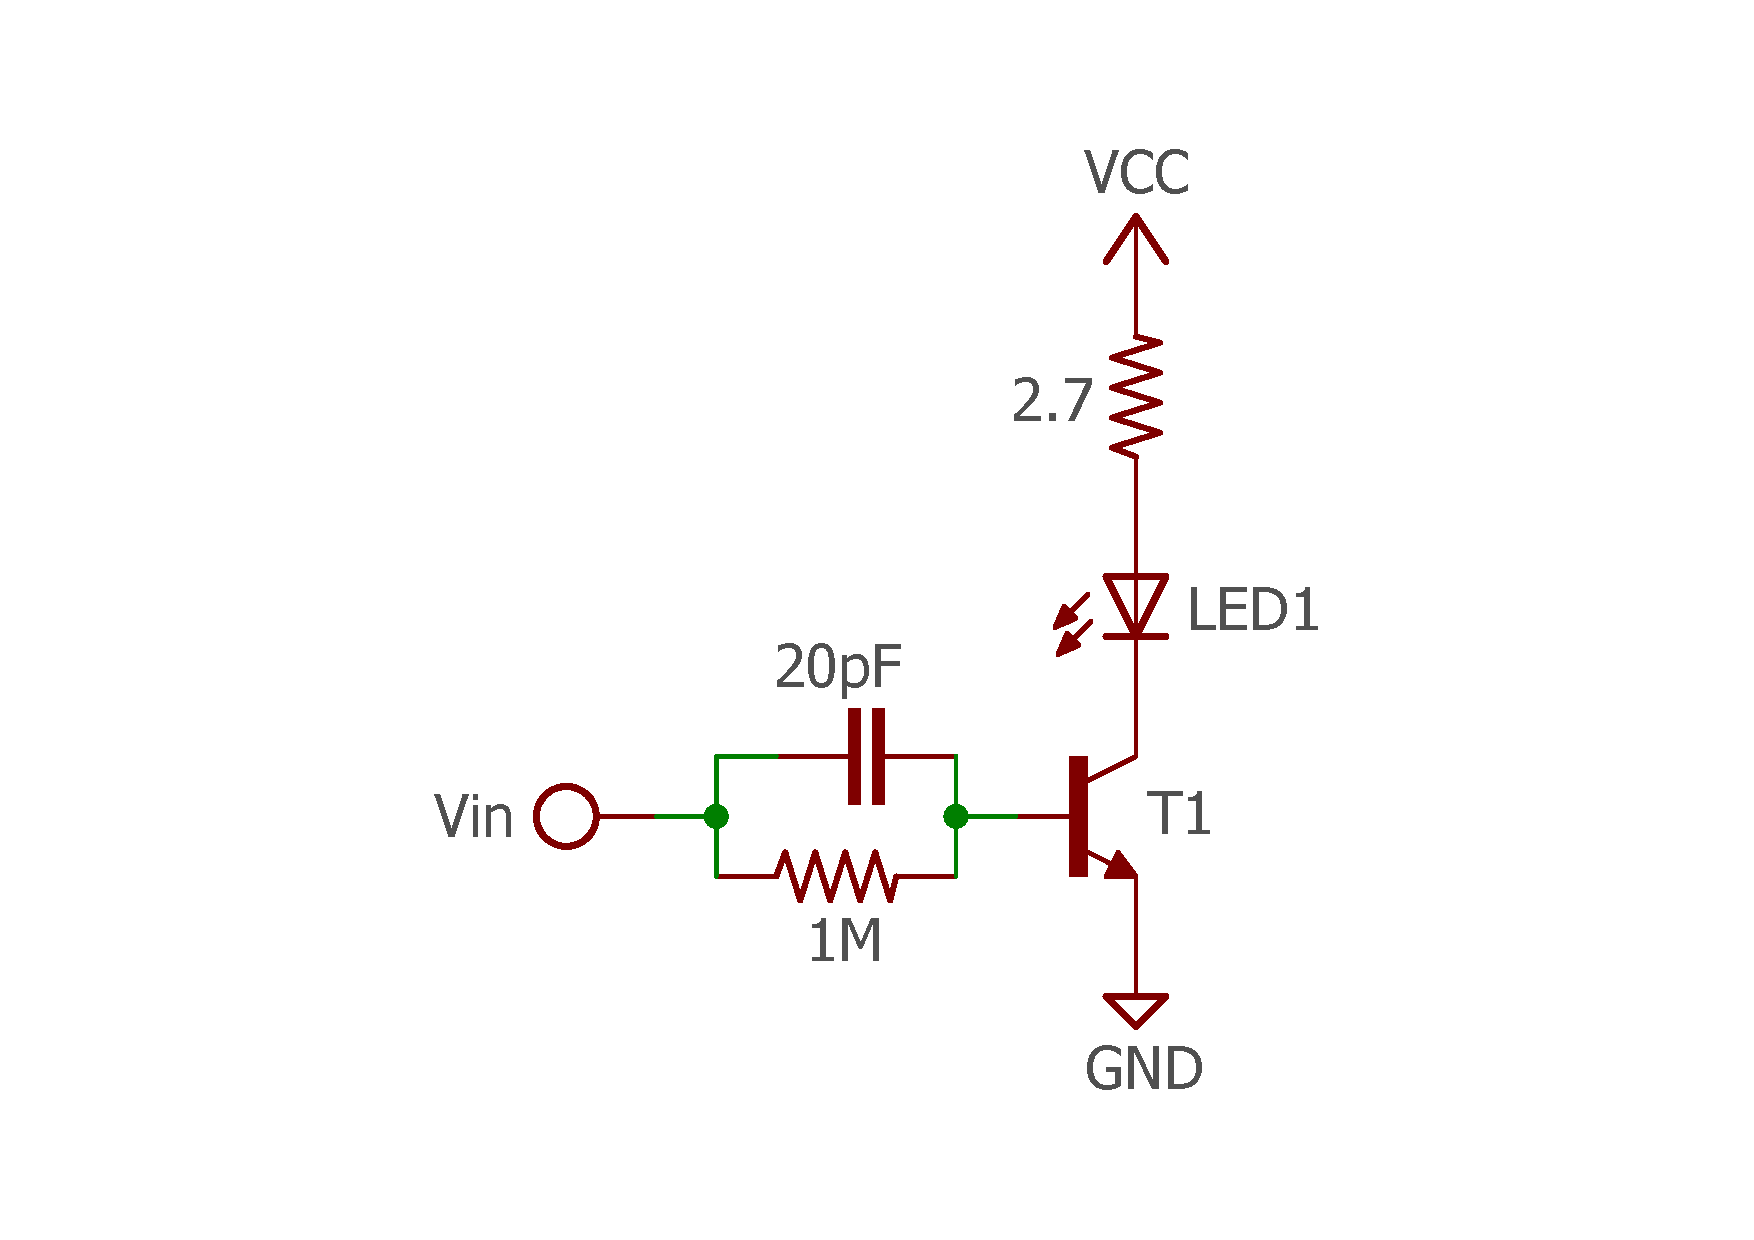
\includegraphics[width=0.7\textwidth, trim={2cm 1cm 2cm 2cm}, clip]{circuits/transmitter_fail0.pdf}
			\legend{Fonte: Autores}
		\end{figure}
		
		A saída dessa implementação é mostrada na \autoref{fig_transmitter_lify_circuit_fail0_rl} e não é satisfatória. O primeiro ponto a se notar é que a frequência de operação era baixa, no caso 80kHz - ainda 120kHz abaixo da especificação da velocidade da camada PHY I. Um segundo ponto observado foi o fato de que houve uma resposta de subamortecimento tanto na entrada quanto na saída. Isso ocorre devido a efeitos de capacitância ou no LED ou no transistor de potência.
		
		\begin{figure}[htb]
			\caption{\label{fig_transmitter_lify_circuit_fail0_rl} Comportamento do circuito de transmissão com filtro de ponta de prova em série com a entrada. A onda azul é saída do gerador de funções enquanto a onda amarela é a tensão submetida ao LED. Observa-se o comportamento de subamortecimento em ambas.}
			\centering		%  trim={<left> <lower> <right> <upper>} 
			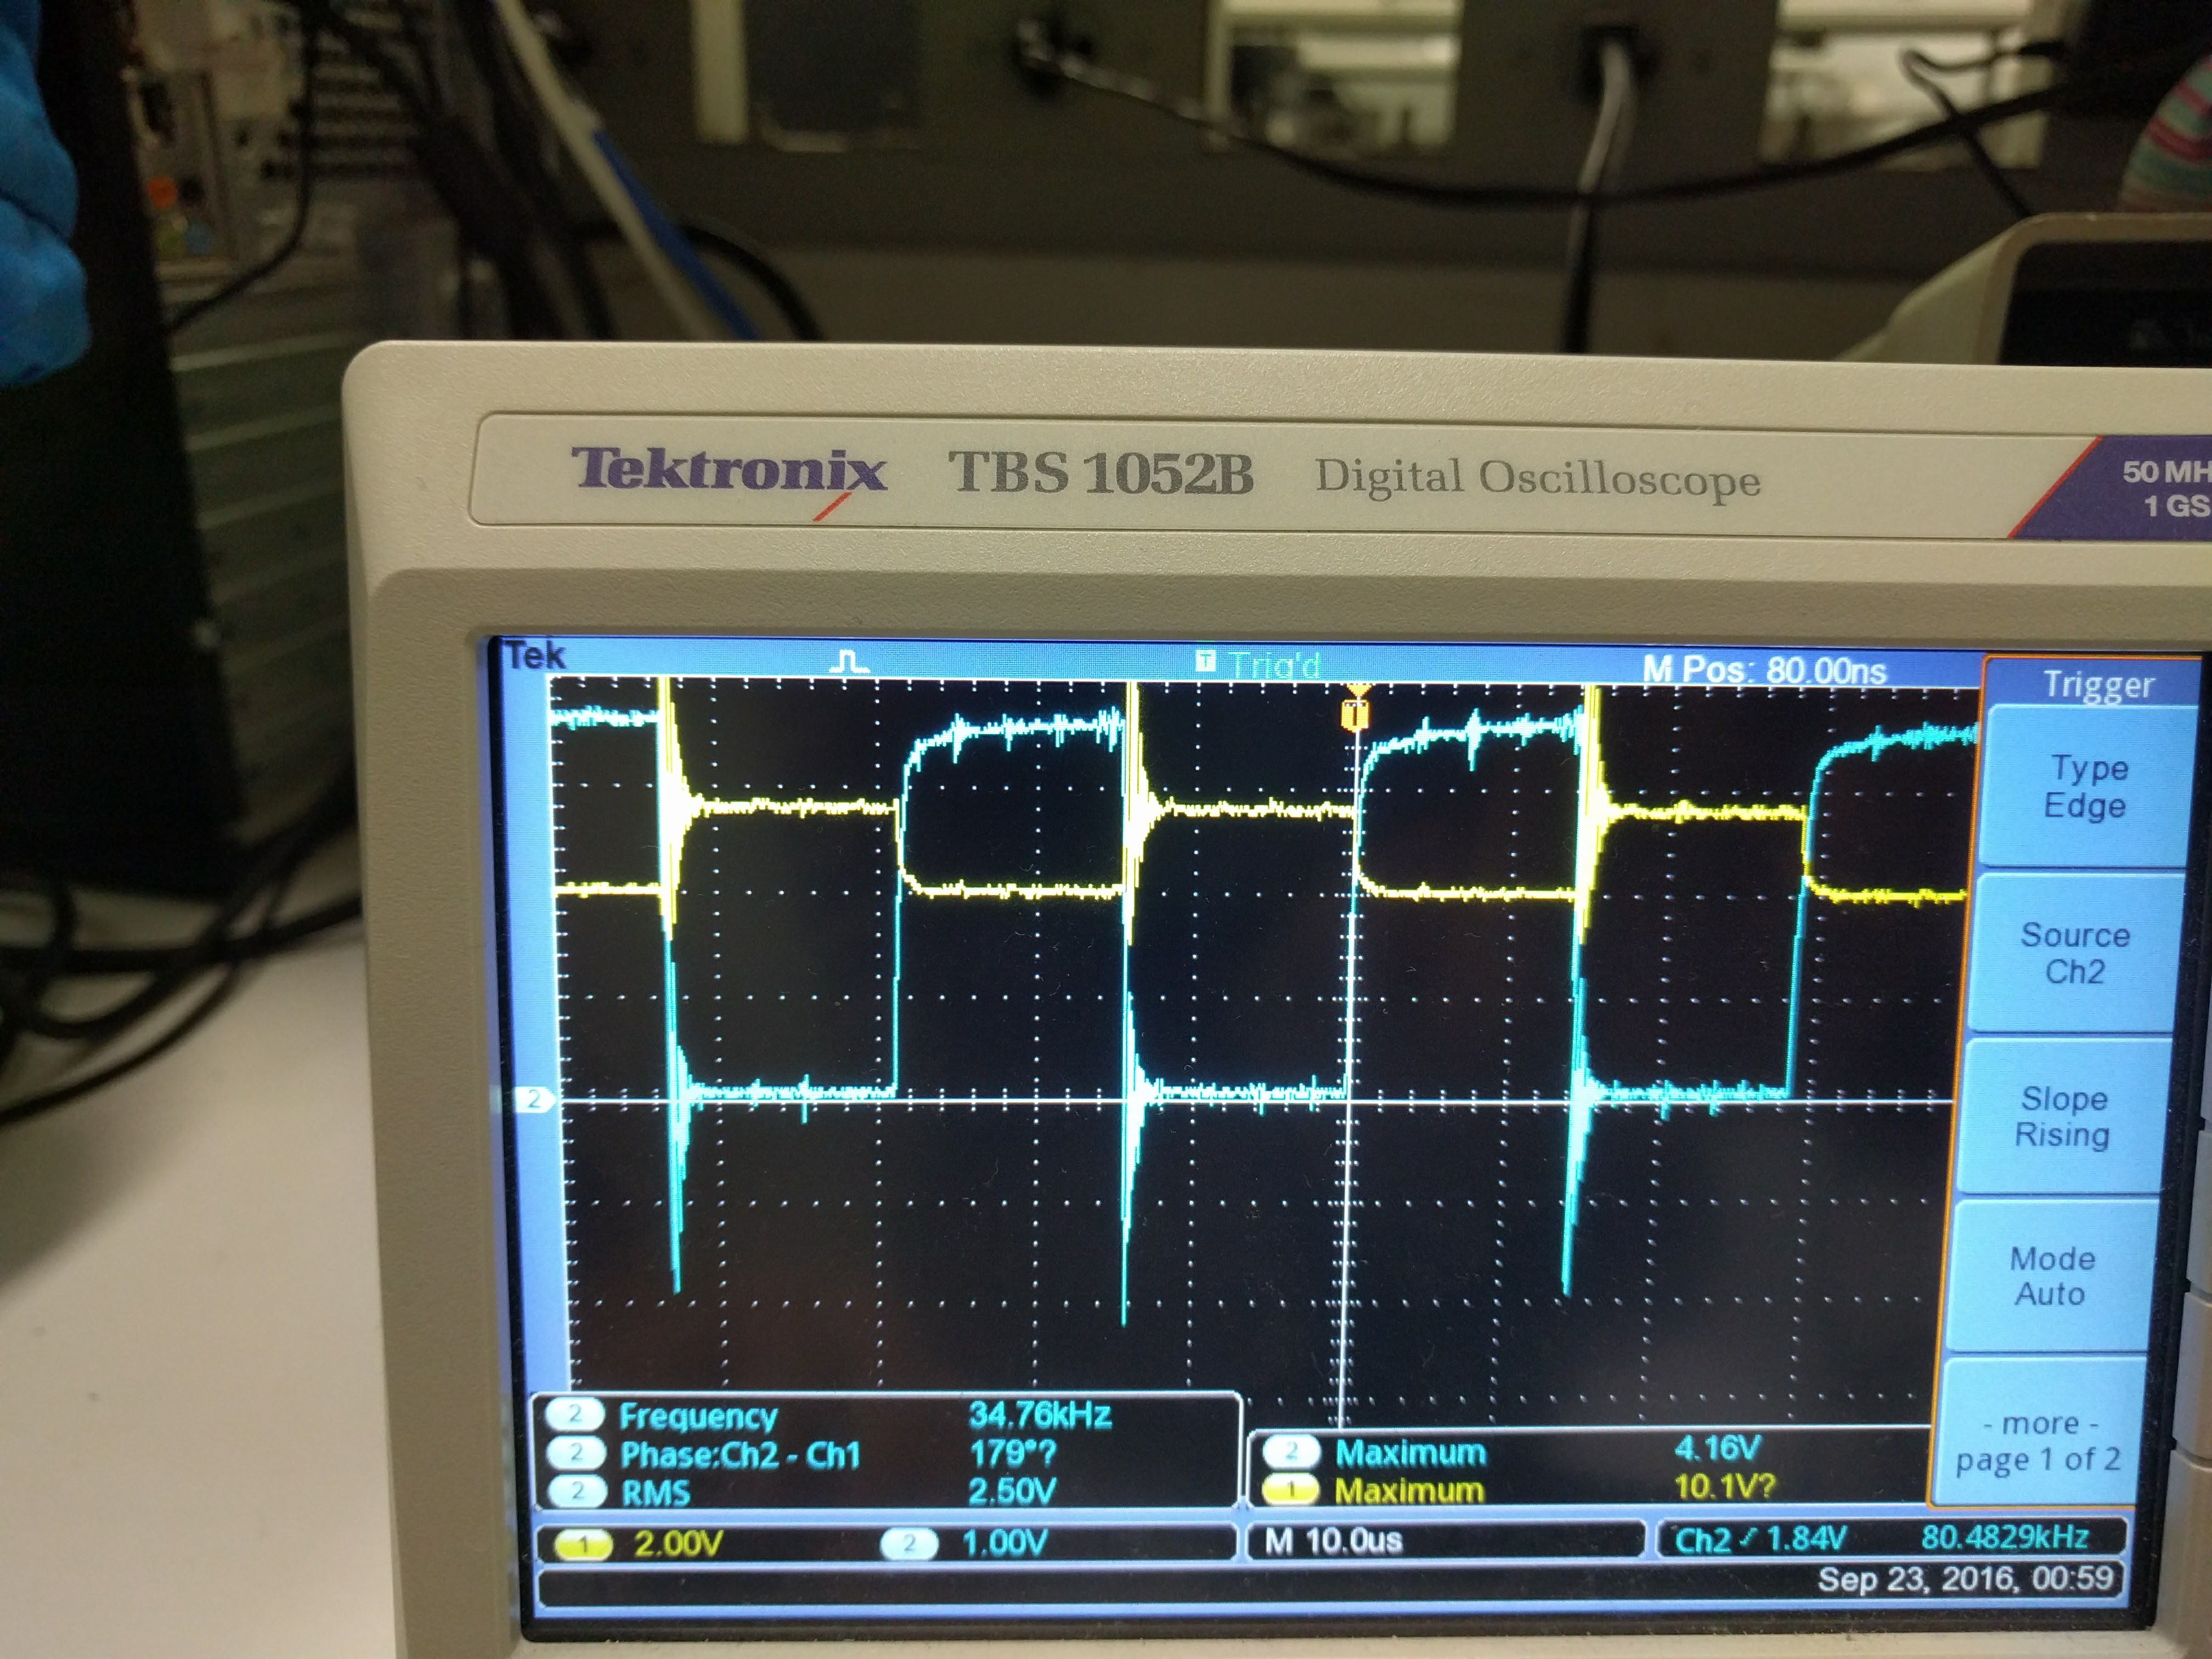
\includegraphics[width=0.7\textwidth, trim={30cm 0cm 2cm 40cm}, clip]{circuits/photos/TX_probe_result.jpg}
			\legend{Fonte: Autores}
		\end{figure}
	
		Ambos os componentes contém esse valor. O transistor de potência possui capacitância devido a separação de suas placas. Seu valor é significativo e é até especificado na datasheet. Para o IRLZ14, a capacitância de entrada é 400pF e de saída 170pF. Esses valores devem ser levados em conta ao polarizar tal componente. 

		No caso do LED, esse comportamento é mais complexo. A frequências altas, seu chaveamento cria um capacitor entre seus terminais, devido a sua arquitetura semicondutora. É possível observar esse comportamento capacitivo tanto em um LED de baixa potência quando de alta. Na prática, a tensão sob o LED não diminui acompanhando a tensão submetida a ele, e isso causa o comportamento indesejável visto.		
		
		Em um teste unitário, foi observado o comportamento do chaveamento de um resistor $R_{L}$ a 200kHz, removendo completamente o LED do sistema. A saída observada era exatamente igual a entrada. Colocando um LED em série com o resistor adicionava o comportamento subamortecido, portanto conclui-se que essa anomalia é atribuida ao LED.
				
		\begin{figure}[htb]
			\caption{\label{fig_transmitter_lify_circuit_fail1_r1} Operação de circuito transmissor. A onda amarela representa voltagem no LED sem filtro de ponta de prova em frequências mais altas. O gerador de funções é medido e gera a forma de onda verde.}
			\centering		%  trim={<left> <lower> <right> <upper>} 
			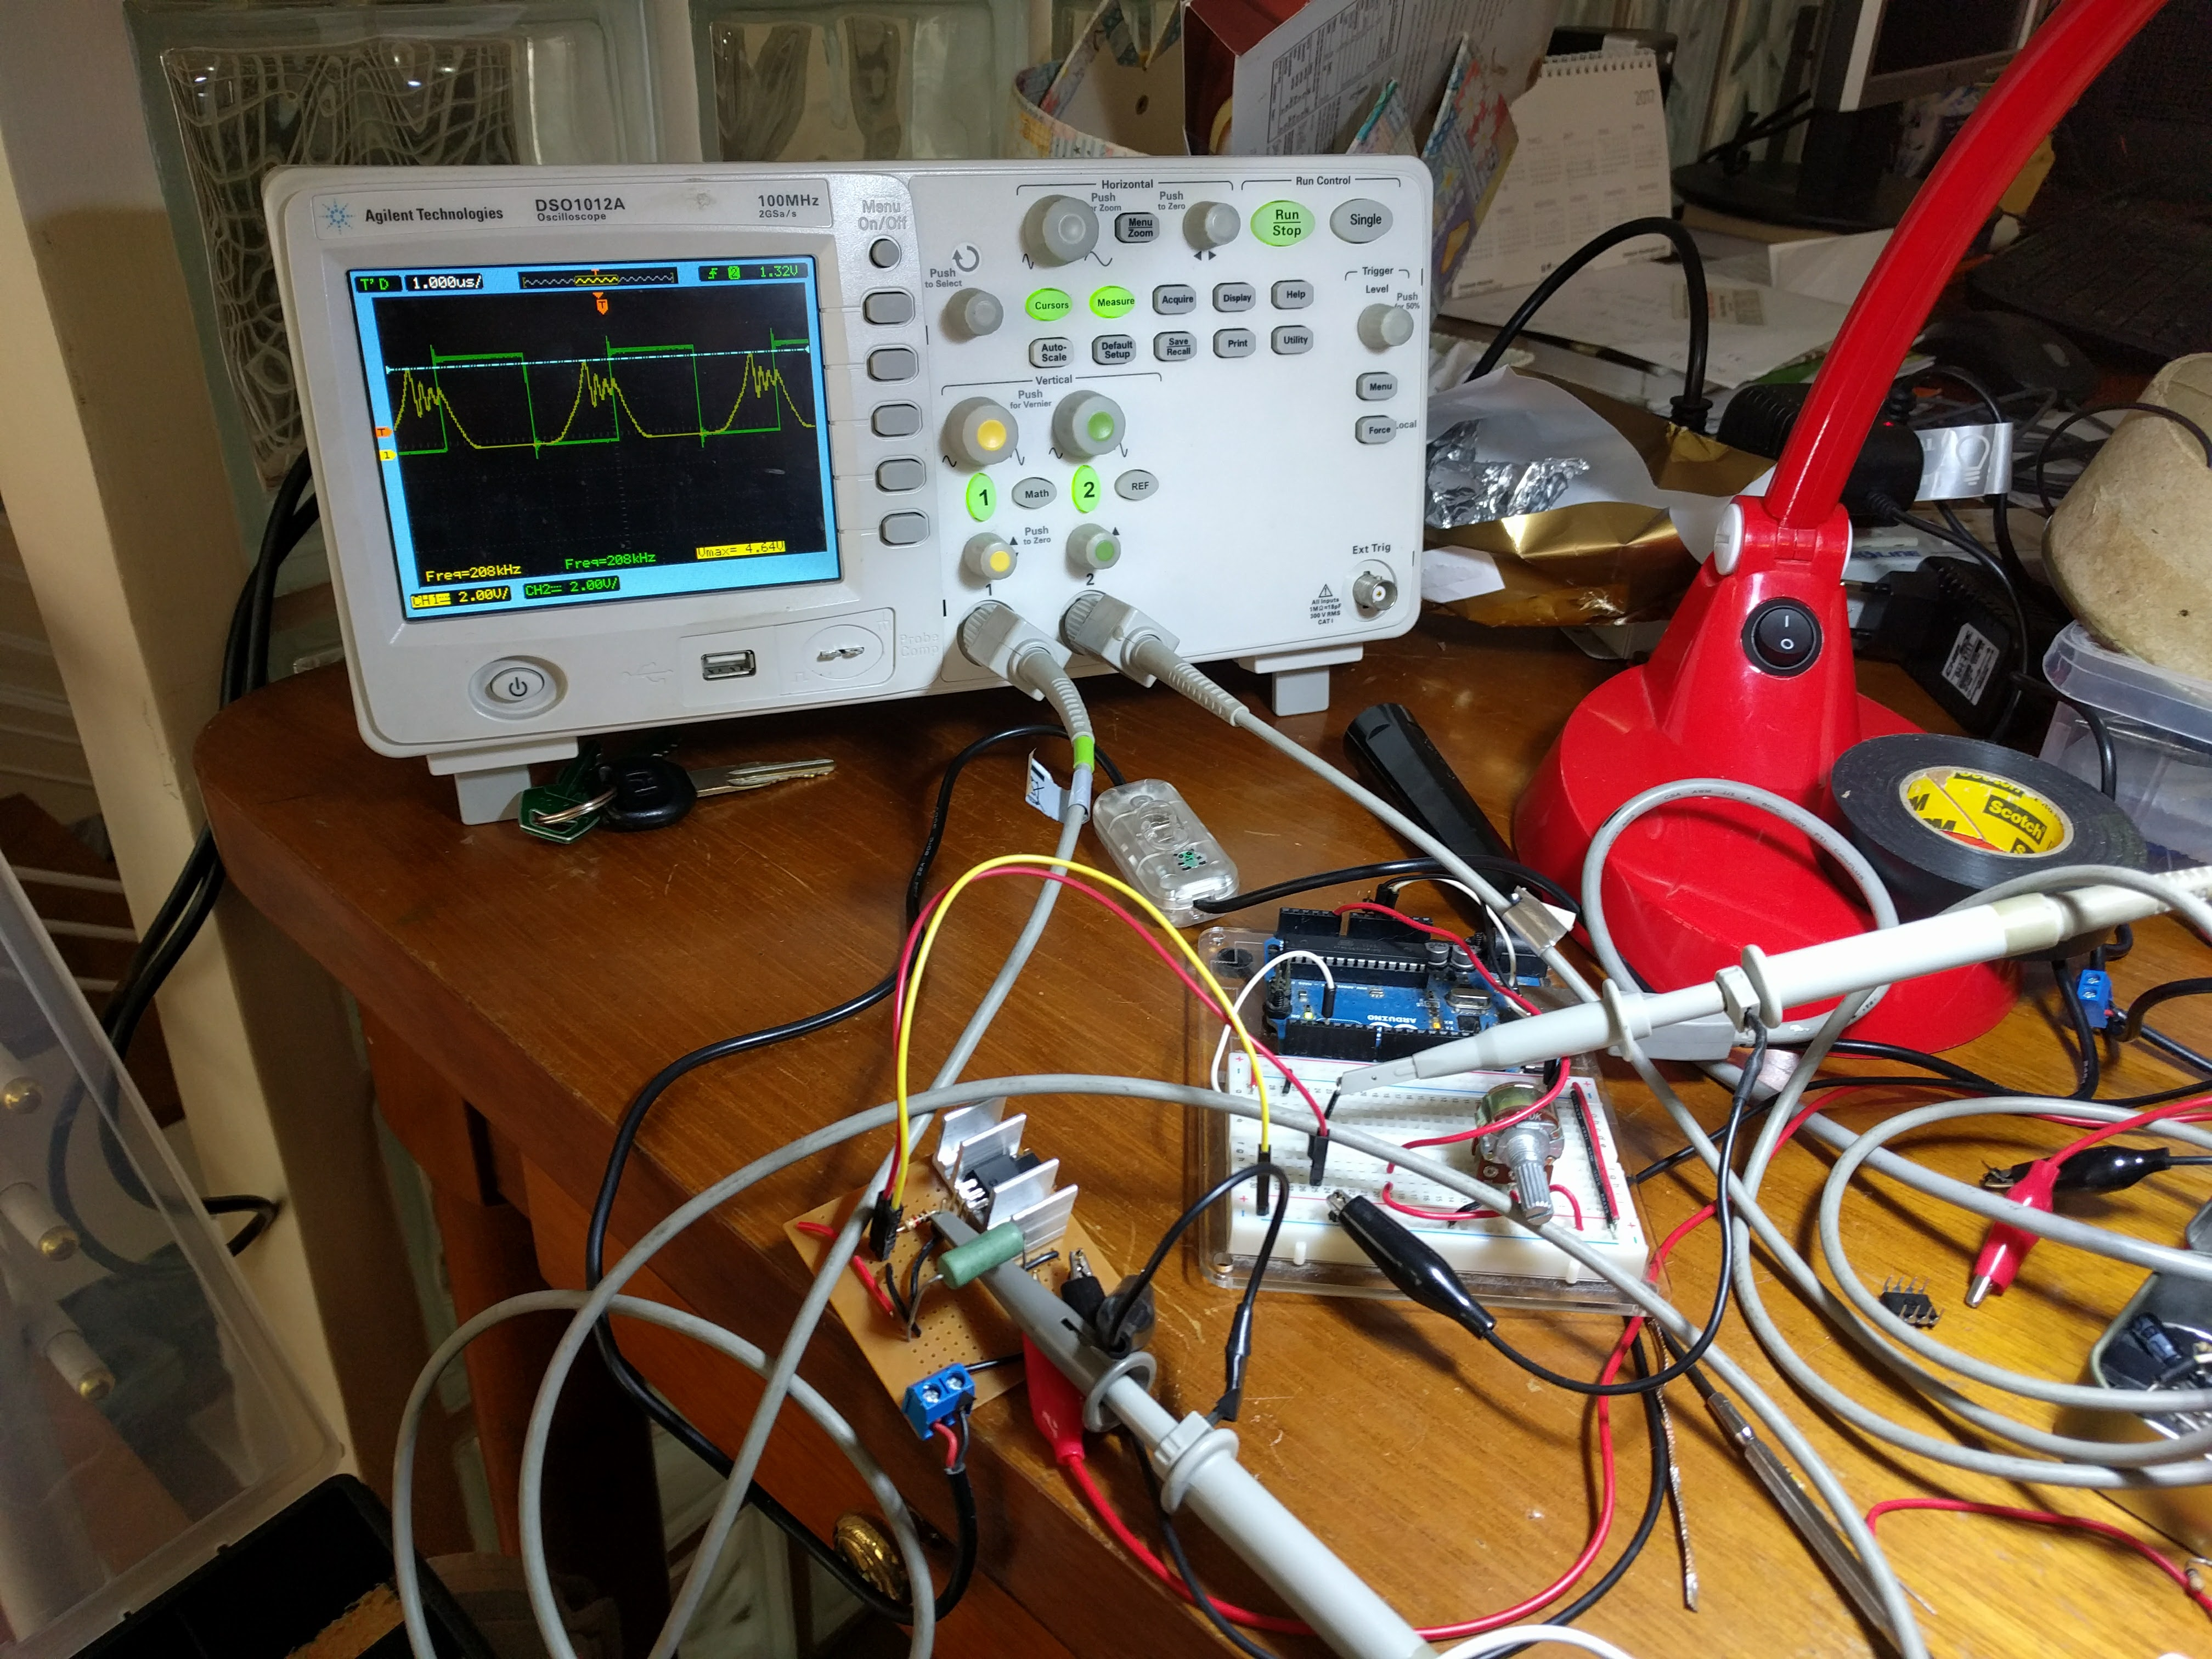
\includegraphics[width=0.7\textwidth, trim={20cm 15cm 50cm 10cm}, clip]{circuits/photos/TX_200k_without_filter.jpg}
			\legend{Fonte: Autores}
		\end{figure}
		
		\paragraph{Aumento da Frequência}
		
		O aumento da frequência de operação a $f_{OP} = 200kHz$ causa um subamortecimento substancialmente maior. Observa-se na \autoref{fig_transmitter_lify_circuit_fail1_r1}, que provém de circuito sem o filtro da ponta de prova na \autoref{fig_transmitter_lify_circuit_fail1}.
		
		\begin{figure}[htb]
			\caption{\label{fig_transmitter_lify_circuit_fail1} Circuito de transmissão de}
			\centering		%  trim={<left> <lower> <right> <upper>} 
			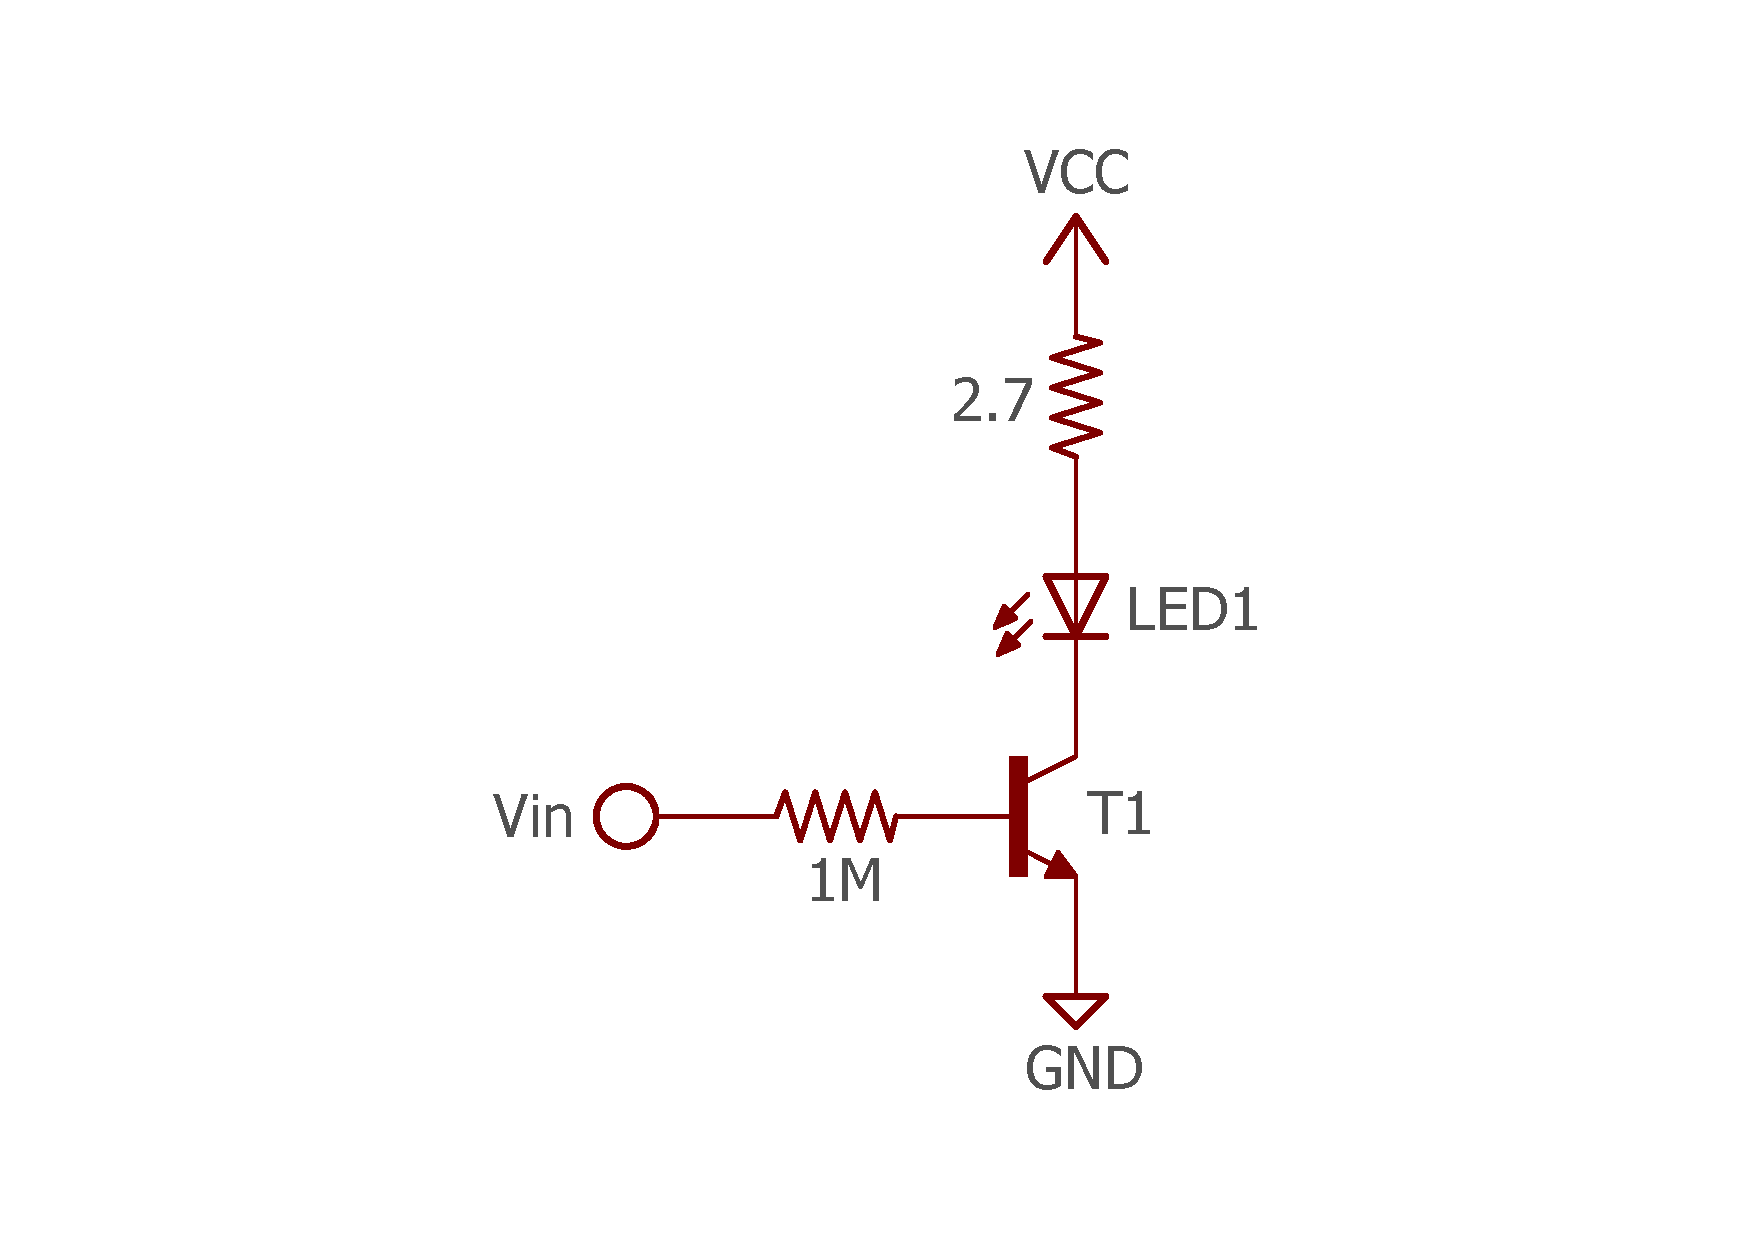
\includegraphics[width=0.7\textwidth, trim={2cm 1cm 2cm 1cm}, clip]{circuits/transmitter_fail1.pdf}
			\legend{Fonte: Autores}
		\end{figure}
		
		Nesse caso é muito mais evidente o amortecimento visto na onda. Atribui-se esse comportamento a componente capacitiva ao chavear o LED. No entanto, observa-se que não há feedback do circuito na saída do gerador de funções, fato observado na última versão do circuito. O capacitor colocado adicionava um nível de complexidade desnecessário ao circuito, pois se carregava com oscilação da entrada. A forma de onda gerada em si era boa, mas os picos de voltagem gerados no início da onda colocavam os componentes em risco.
		
		A forma de onda gerada por esse circuito é difícil de ser usada, pois não preserva o período da onda de entrada. Mesmo com muitos filtros no receptor não é possível corrigir a essa diferença.
		
		\paragraph{Final - Filtro Passa-Altas}
				
		\begin{figure}[htb]
			\caption{\label{fig_transmitter_lify_circuit_final} Circuito de transmissão de dados LiCy.}
			\centering		%  trim={<left> <lower> <right> <upper>} 
			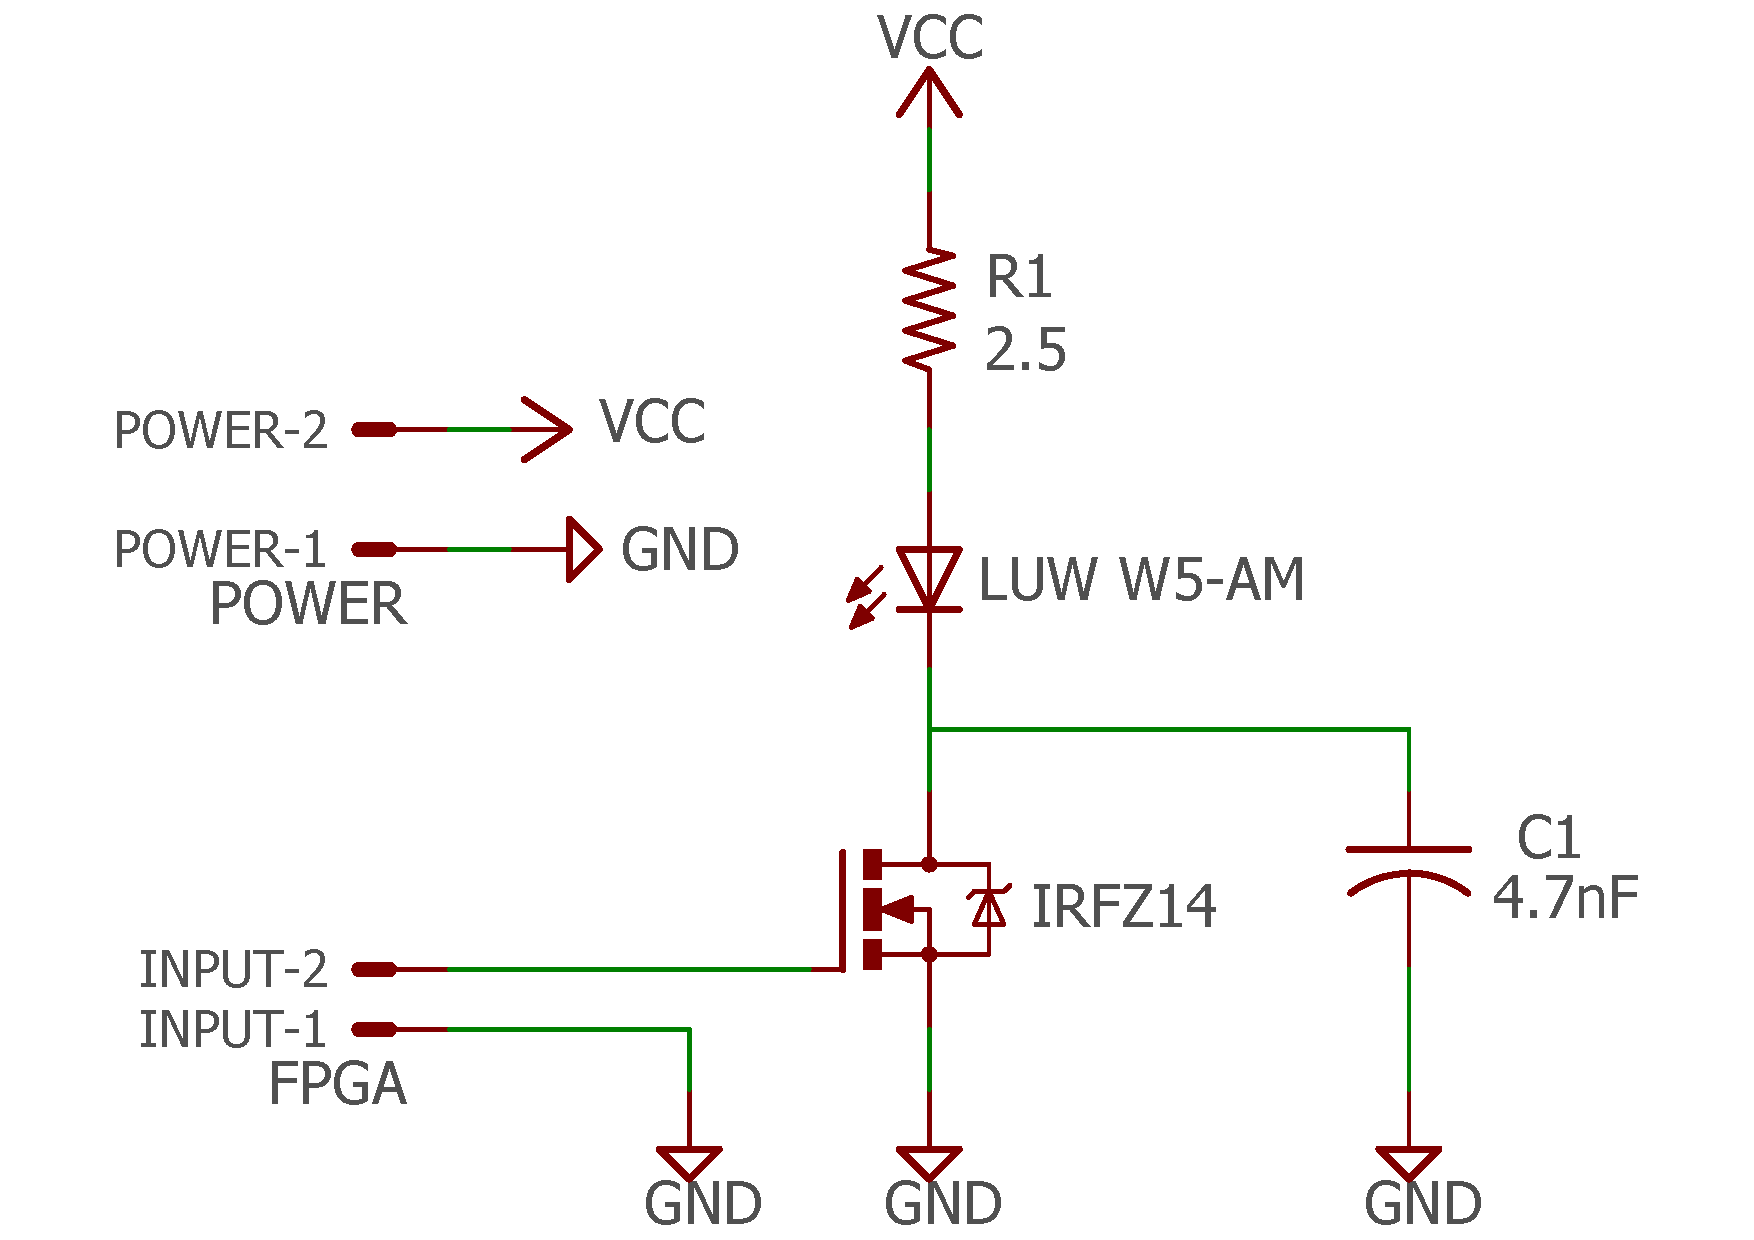
\includegraphics[width=0.7\textwidth, trim={2cm 0cm 2cm 0cm}, clip]{circuits/transmitter_lify.pdf}
			\legend{Fonte: Autores}
		\end{figure}
		
		\begin{figure}[htb]
			\caption{\label{fig_transmitter_lify_circuit_final_r1} Forma de onda após adicionar um capacitor que age como filtro passa-altas. Está defasada em 180$\degree$. }
			\centering		%  trim={<left> <lower> <right> <upper>} 
			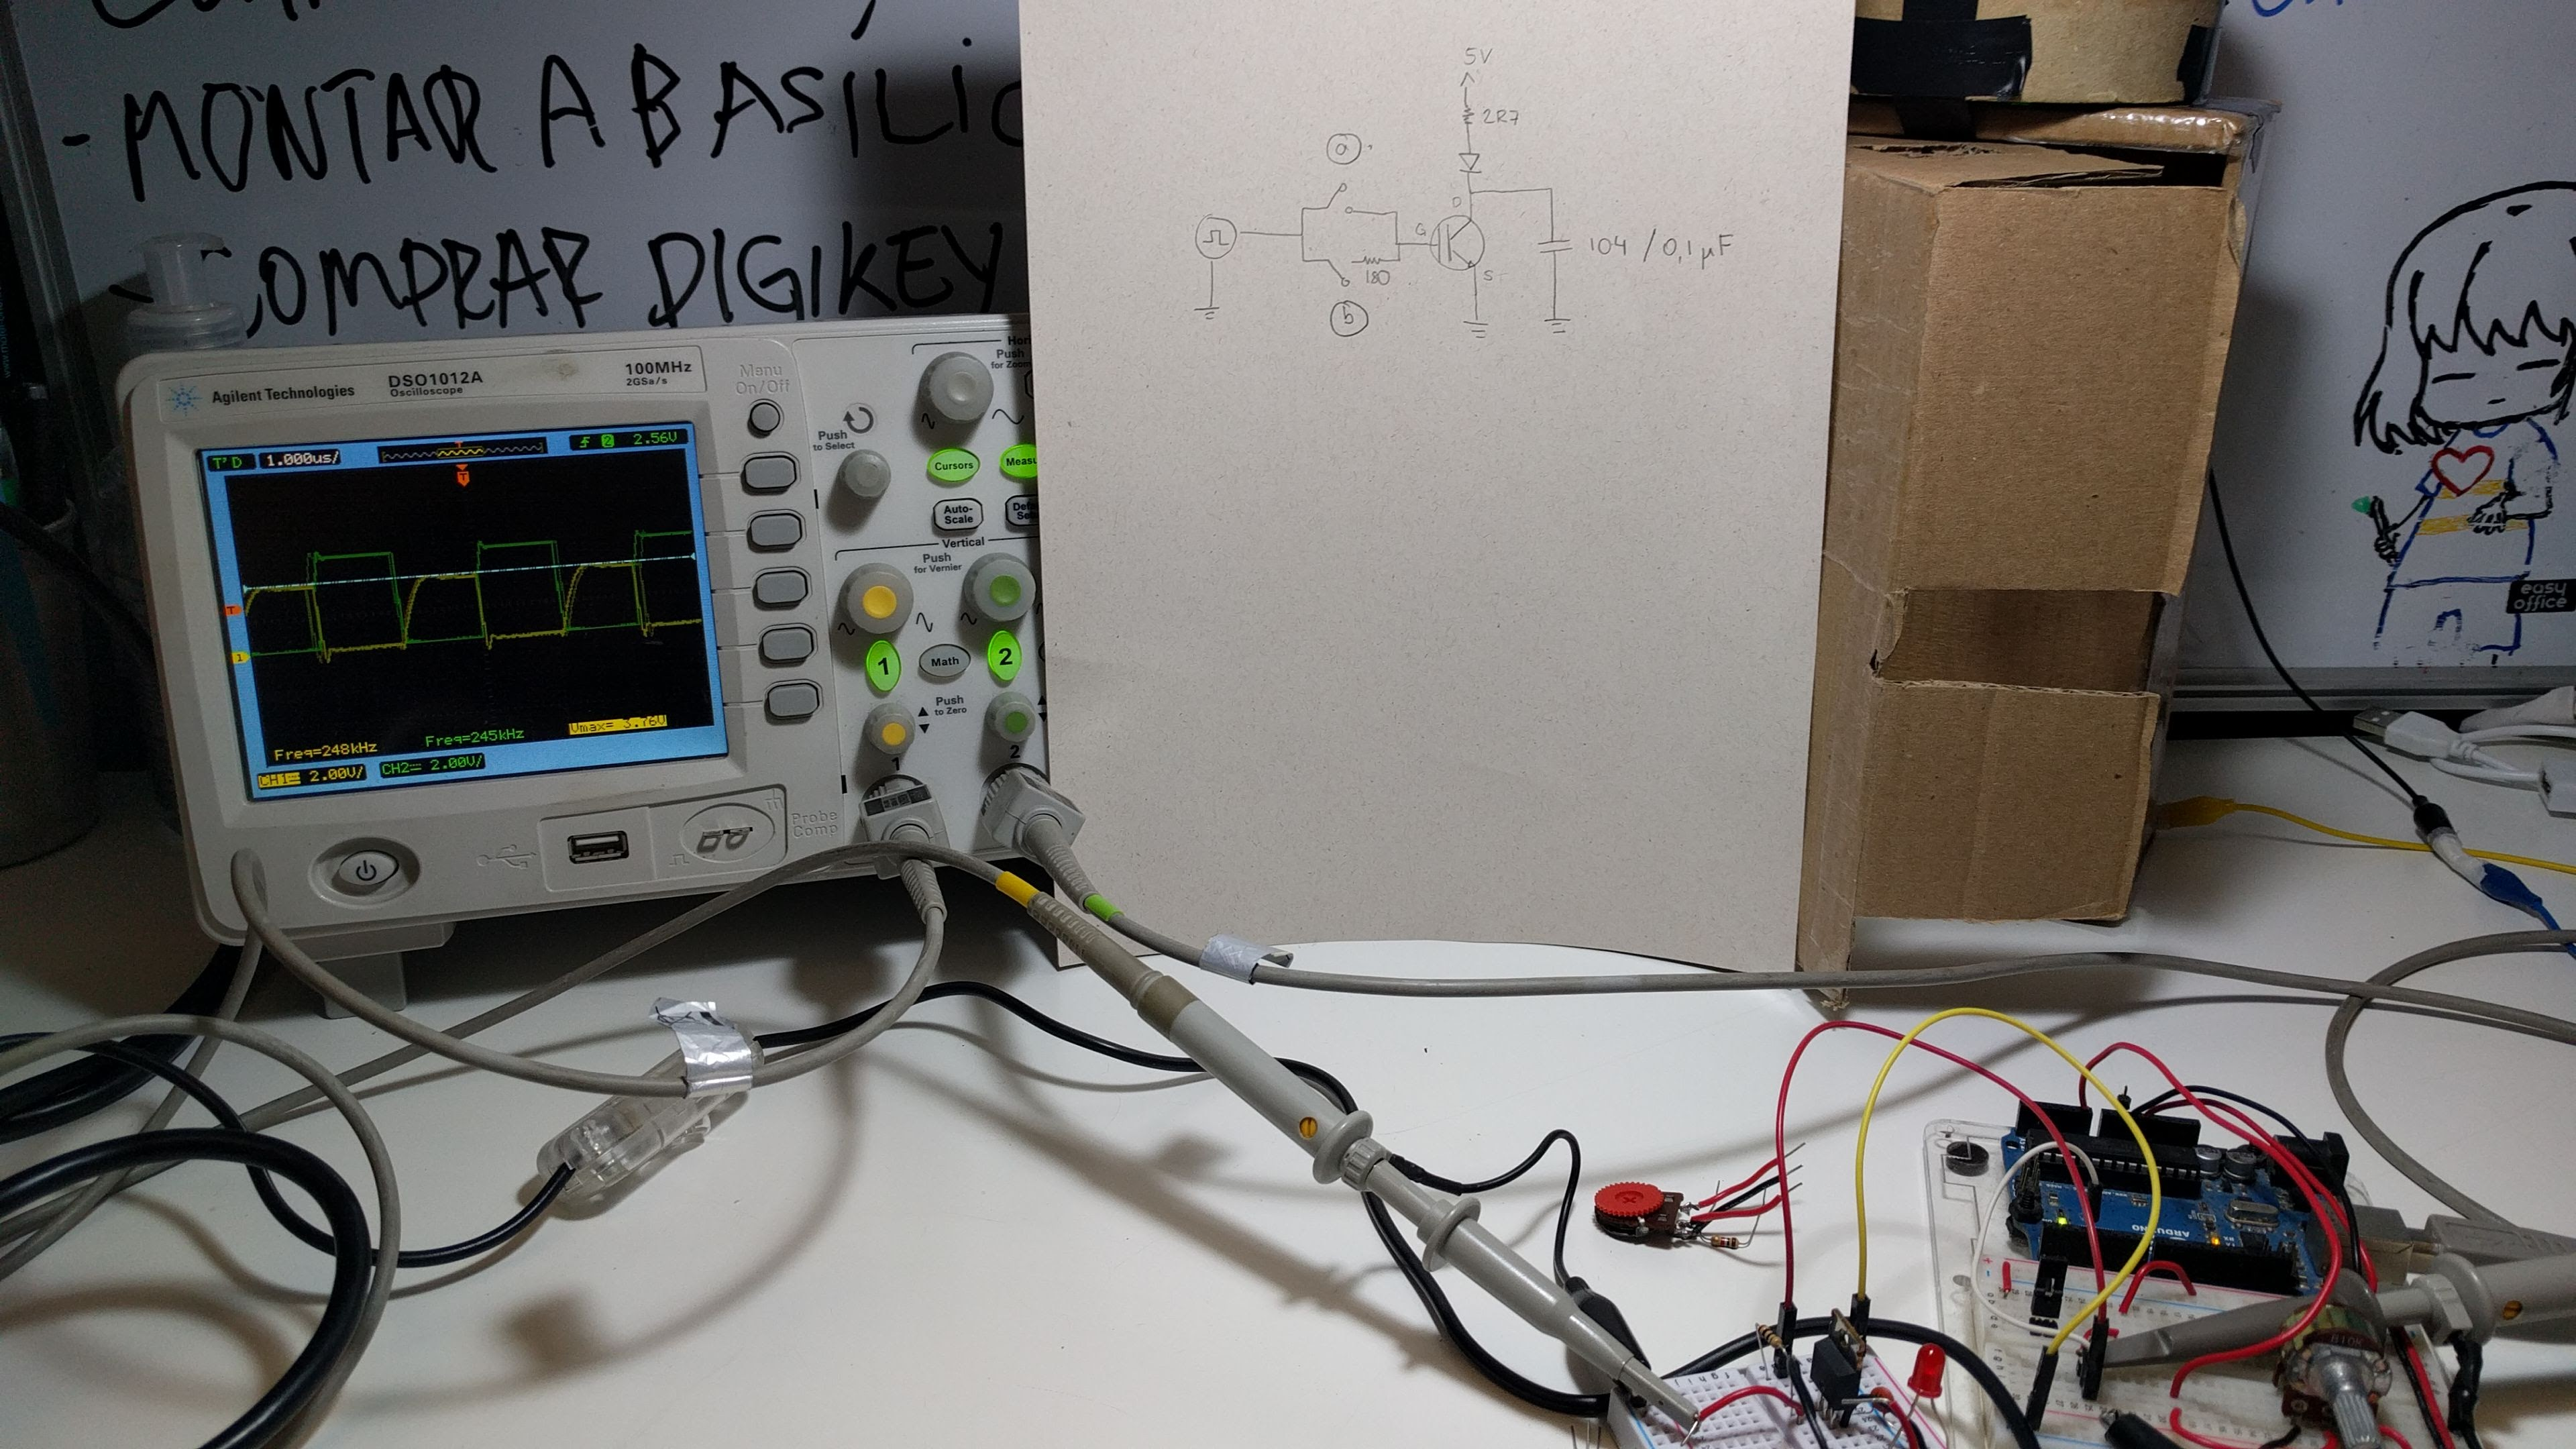
\includegraphics[width=0.7\textwidth, trim={5cm 30cm 20cm 20cm}, clip]{circuits/photos/TX_200k_with_filter.jpeg}
			\legend{Fonte: Autores}
		\end{figure}

		Por fim, realiza-se a correção dessa componente utilizando um capacitor entre os terminais da Source do MOSFET e GND (observado em \autoref{fig_transmitter_lify_circuit_final}). Esse capacitor atua como filtro passa-altas e remove a componente AC da saída para o LED. O comportamento não fica exatamente igual à entrada, mas fica satisfatório pois o período é muito similar, chaveando o LED corretamente. A forma de onda resultante pode ser observada em \autoref{fig_transmitter_lify_circuit_final_r1}. Está defasada em 180$\degree$.
	
		\subsection{Receptor}
		
		A recepção será feita utilizando os conceitos apresentados nas seções \ref{method-hard-photodiode}, \ref{method-hardware-conv-ad}, \ref{method-hardware-highpass-filter}, \ref{method-hardware-dc-bias};
		
		\subsubsection{Recepção Luminosa}
		
		Para o recebimento luminoso, foi utilizado um circuito da \textbf{APPLICATION NOTES} da \citeonline{datasheet-opa380}, simplificado e esquematizado na \autoref{fig_transimpedance_amp_simple}. O valor de R1 foi escolhido como 1M$\Omega$.
		
		\begin{figure}[htb]
			\caption{\label{fig_receiver_lify_circuit_fail0_r1} Saída do Amplificador de Transimpedância (amarela) para uma entrada luminosa de 200kHz (verde).}
			\centering		%  trim={<left> <lower> <right> <upper>} 
			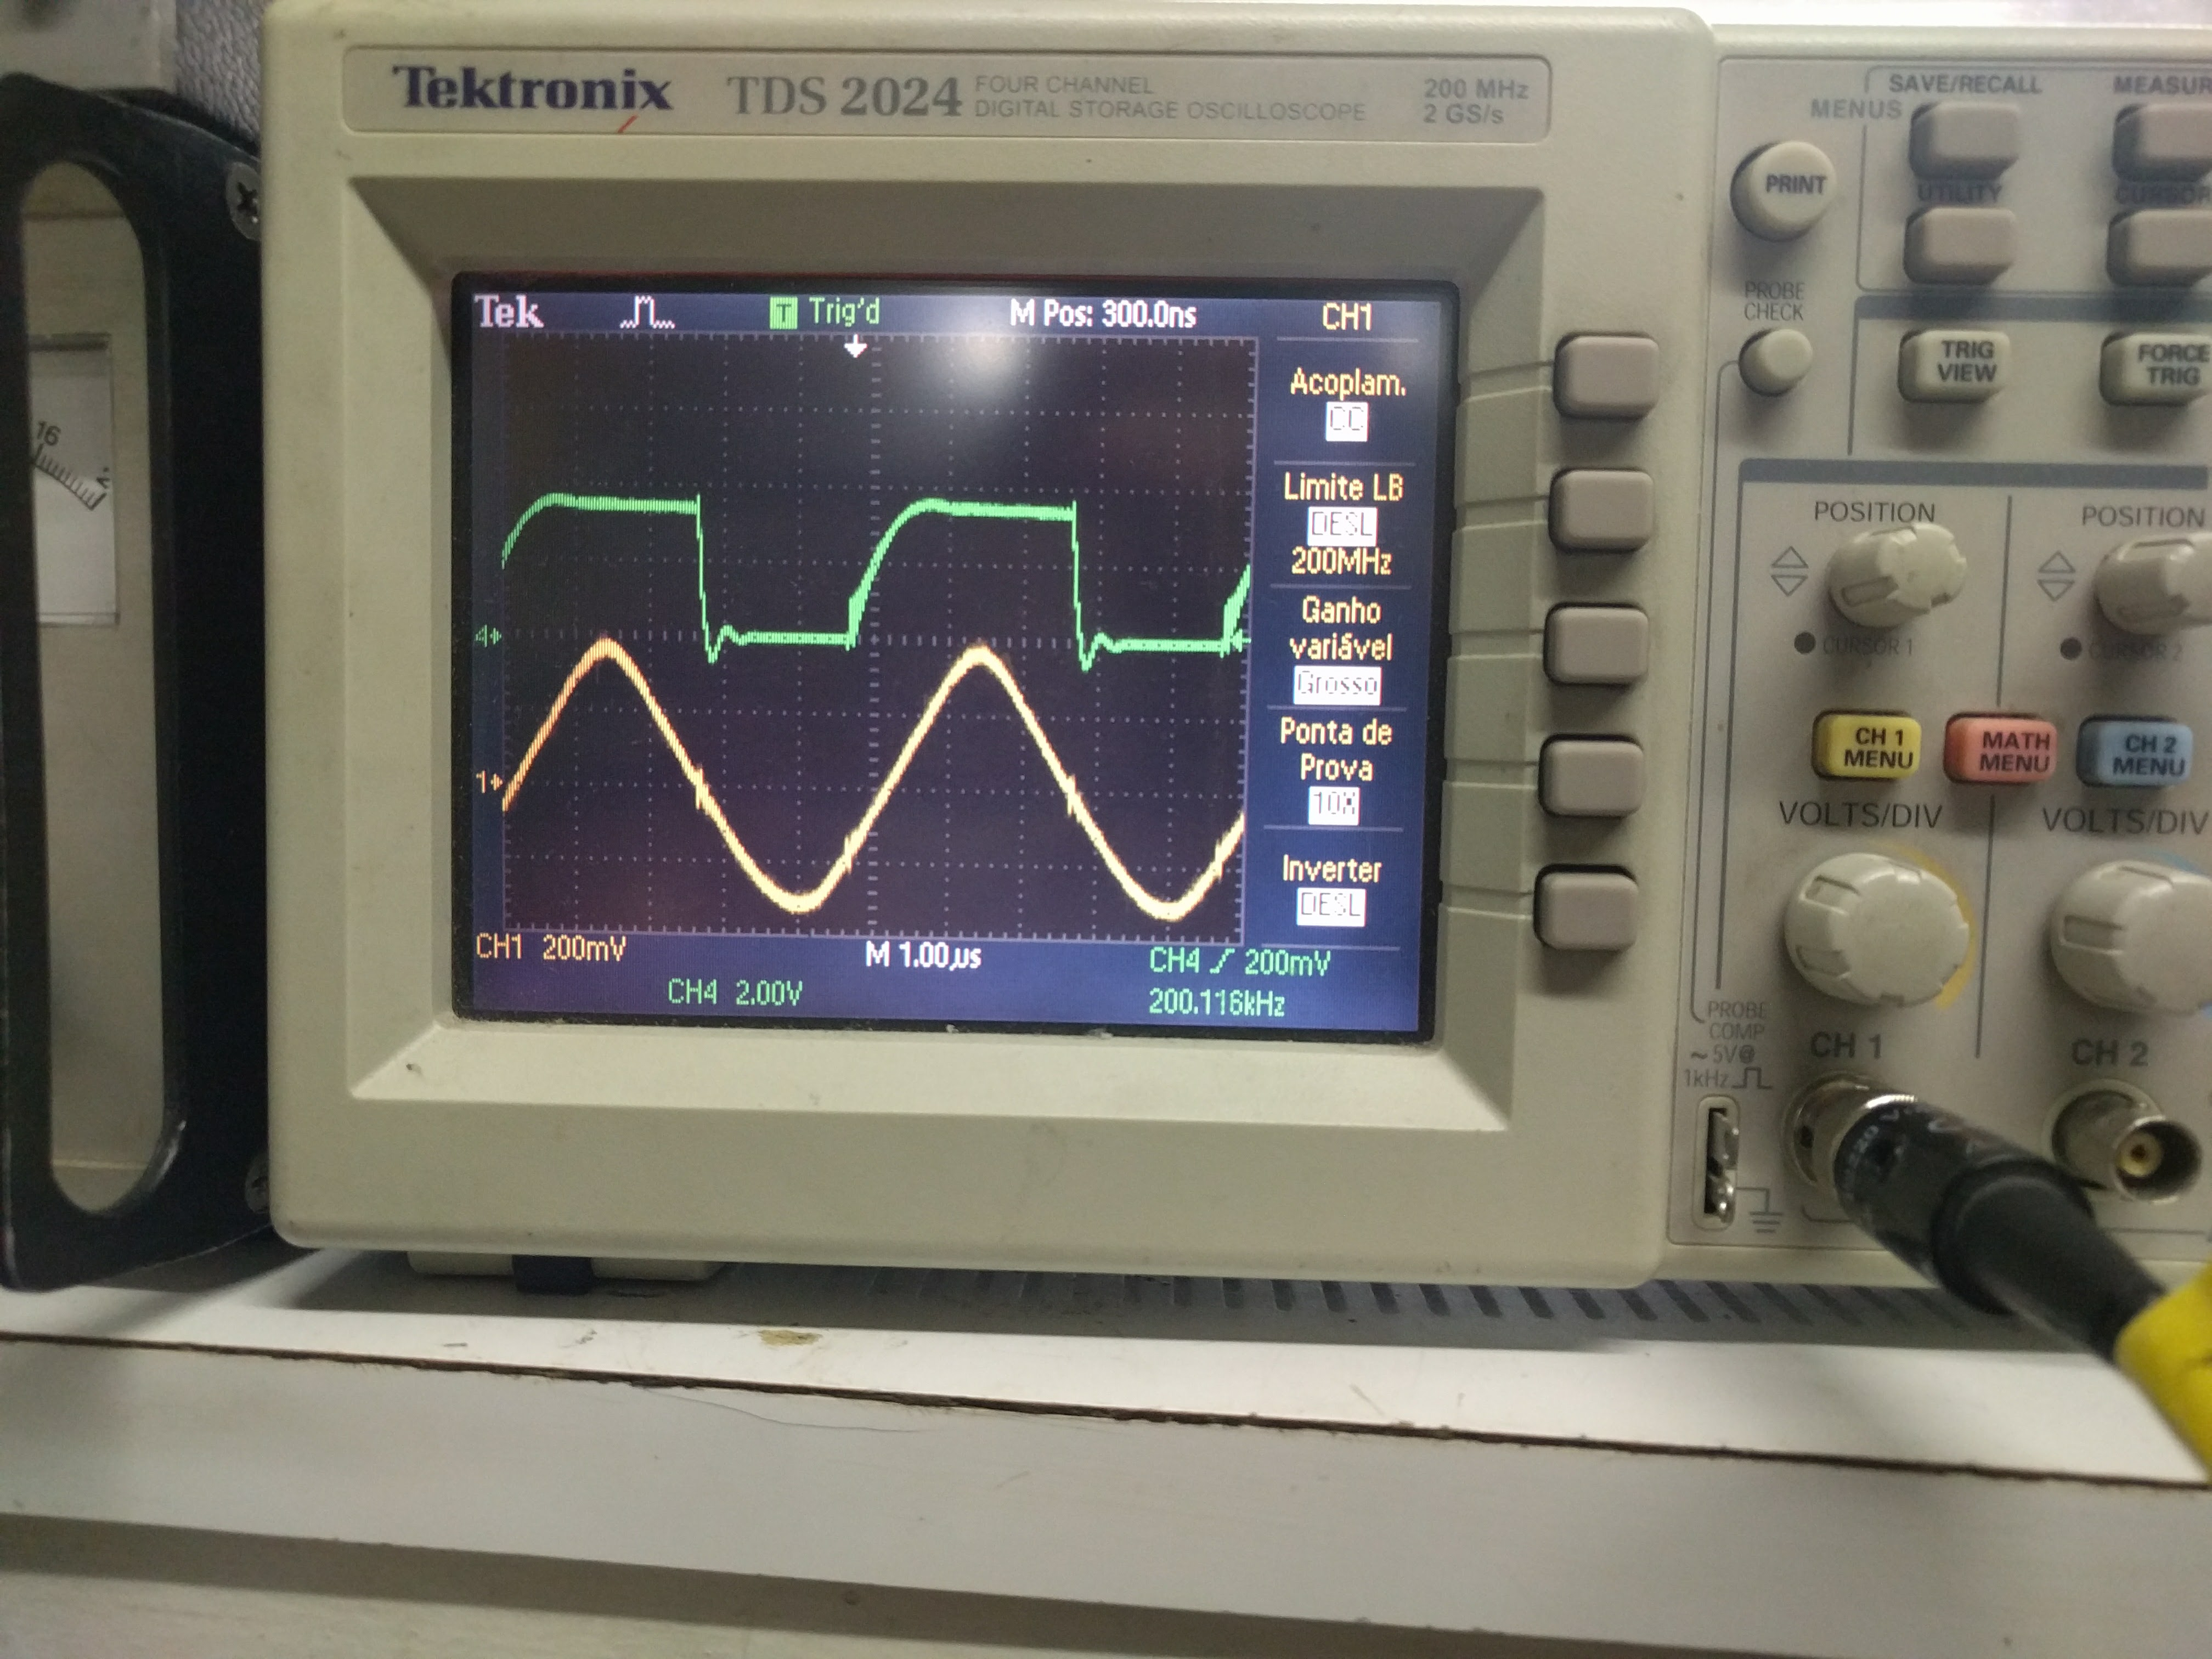
\includegraphics[width=0.7\textwidth, trim={5cm 30cm 90cm 20cm}, clip]{circuits/photos/RX_TIA_result.jpg}
			\legend{Fonte: Autores}
		\end{figure}
		
		\subsubsection{Conversor Analógico-Digital}
		
		O conversor analógico-digital foi integrado 
	
		\begin{figure}[htb]
			\caption{\label{fig_receiver_lify_circuit_final} Circuito esquemático final.}
			\centering
			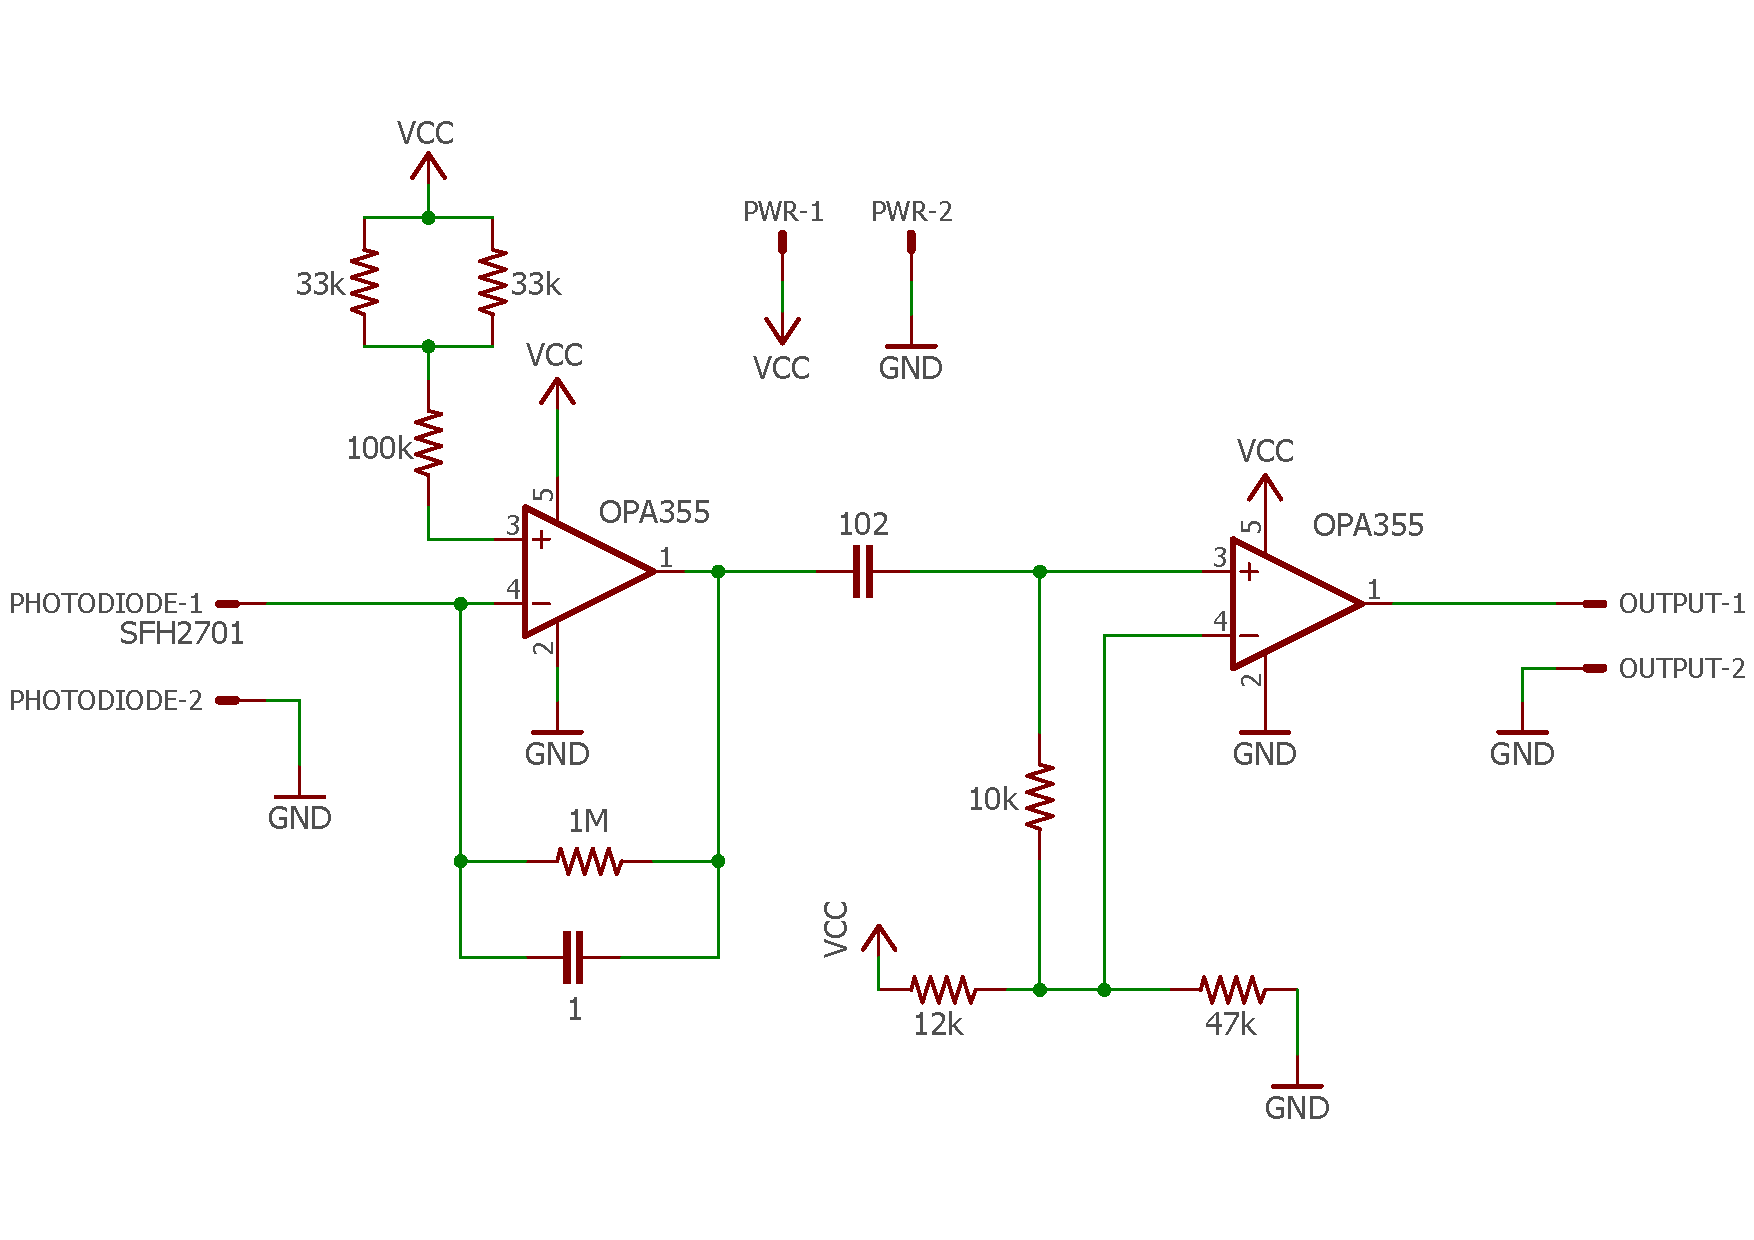
\includegraphics[width=1\textwidth, trim={0cm 1cm 0cm 1cm}, clip]{circuits/receiver_lify_final.pdf}
			\legend{Fonte: Autores}
		\end{figure}
	
		\section{Software}
		Com os dados codificados, enviados via luz, recebidos via luz e decodificados, é possível realizar 